\documentclass[11pt]{article}
\headheight = 14pt
% packages
\usepackage{physics}
% margin spacing
\usepackage[top=1in, bottom=1in, left=0.5in, right=0.5in]{geometry}
\usepackage{hanging}
\usepackage{amsfonts, amsmath, amssymb, amsthm}
\usepackage{systeme}
\usepackage[none]{hyphenat}
\usepackage{fancyhdr}
\usepackage[nottoc, notlot, notlof]{tocbibind}
\usepackage{graphicx}
\graphicspath{{./images/}}
\usepackage{float}
\usepackage{siunitx}
\usepackage{esint}
\usepackage{cancel}
\usepackage{enumitem}
\usepackage{tikz-cd}

% colors
\usepackage{xcolor}
\definecolor{p}{HTML}{FFDDDD}
\definecolor{g}{HTML}{D9FFDF}
\definecolor{y}{HTML}{FFFFCF}
\definecolor{b}{HTML}{D9FFFF}
\definecolor{o}{HTML}{FADECB}
%\definecolor{}{HTML}{}

% \highlight[<color>]{<stuff>}
\newcommand{\highlight}[2][p]{\mathchoice%
  {\colorbox{#1}{$\displaystyle#2$}}%
  {\colorbox{#1}{$\textstyle#2$}}%
  {\colorbox{#1}{$\scriptstyle#2$}}%
  {\colorbox{#1}{$\scriptscriptstyle#2$}}}%

% header/footer formatting
\pagestyle{fancy}
\fancyhead{}
\fancyfoot{}
\fancyhead[L]{MTG4303}
\fancyhead[C]{HW 1}
\fancyhead[R]{Sai Sivakumar}
\fancyfoot[R]{\thepage}
\renewcommand{\headrulewidth}{1pt}

% paragraph indentation/spacing
\setlength{\parindent}{0cm}
\setlength{\parskip}{5pt}
\renewcommand{\baselinestretch}{1.25}

% extra commands defined here
\newcommand{\br}[1]{\left(#1\right)}
\newcommand{\sbr}[1]{\left[#1\right]}
\newcommand{\cbr}[1]{\left\{#1\right\}}

% bracket notation for inner product
\usepackage{mathtools}

\DeclarePairedDelimiterX{\abr}[1]{\langle}{\rangle}{#1}

\DeclareMathOperator{\Span}{span}
\DeclareMathOperator{\card}{card}
\DeclareMathOperator{\Int}{Int}
\DeclareMathOperator{\Bd}{Bd}
\DeclareMathOperator{\id}{id}

% set page count index to begin from 1
\setcounter{page}{1}

\begin{document}
\begin{enumerate}
    \item (51.1) Show that if $h,h^{\prime}\colon X\to Y$ are homotopic and $k,k^{\prime}\colon Y\to Z$ are homotopic, then $k\circ h$ and $k^{\prime}\circ h^{\prime}$ are homotopic.
    \begin{proof}
        Suppose $h,h^{\prime}\colon X\to Y$ are homotopic and $k,k^{\prime}\colon Y\to Z$ are homotopic. 

        Define the map $H^{\prime}\colon X\times I \to Y\times I$ by $H^{\prime}(x,t) = (H(x,t),t)$. It is clear that this map is continuous because the component maps are continuous. Then the desired homotopy is the map $K\circ H^{\prime} \colon X\times I \to Z$ (continuous because composition of continuous maps are continuous). We have \begin{align*}
            &K\circ H^{\prime}(x,0) = K(H(x,0),0) = K(h(x),0) = k(h(x)) = (k\circ h)(x)\\
            &K\circ H^{\prime}(x,1) = K(H(x,1),1) = K(h^{\prime}(x),0) = k^{\prime}(h^{\prime}(x)) = (k^{\prime}\circ h^{\prime})(x)
        \end{align*}
        as desired, meaning $k\circ h$ and $k^{\prime}\circ h^{\prime}$ are homotopic.
    \end{proof}
    \item (51.3) A space $X$ is said to be \textbf{\textit{contractible}} if the identity map $i_X\colon X\to X$ is nulhomotopic. \begin{enumerate}[label=(\alph*)]
        \item Show that $I$ and $\mathbb{R}$ are contractible.
        \begin{proof}
            Observe that $I$ and $\mathbb{R}$ are both convex, path connected sets. Let $f\colon I\to I$ and $g\colon \mathbb{R}\to \mathbb{R}$ be constant maps. Then the straight line homotopies \begin{align*}
                &F\colon I\times I\to I \text{ given by } F(x,t) = tf(x)+(1-t)x\\
                &G\colon \mathbb{R}\times I\to \mathbb{R} \text{ given by } G(x,t) = tg(x)+(1-t)x
            \end{align*} are continuous; furthermore, $F(x,1) = f(x)$, $G(x,1) = g(x)$, and $F(x,0) = \id_I(x)$, $G(x,0) = \id_\mathbb{R}(x)$.
        \end{proof}
        \item Show that a contractible space is path connected.
        \begin{proof}
            Suppose that $X$ is a contractible space. Let $a,b$ be any two points in $X$. Then for a constant map $f$ on $X$ sending any $x$ to $b$, the identity map is homotopic to this map by some homotopy $F$. Then for any $x$, we can define a path $P_x\colon I\to X$ by $P_x(t) = F(x,t)$, which connects $x$ ($t=0$) to $b$ ($t=1$). So there are paths connecting any $x$ to $b$, and in particular, $P_a$ is a path connecting $a$ to $b$. Since $a,b$ were arbitrary it follows that $X$ is path connected.
        \end{proof}
        \item Show that if $Y$ is contractible, then for any $X$, the set $[X,Y]$ has a single element.
        \begin{proof}
            Suppose $Y$ is contractible and let $X$ be any space. Let $g$ be a constant map on $Y$ mapping $y\in Y$ to $b$. There is a homotopy $F\colon Y\times I\to Y$ from the identity map on $Y$ to the map $g$ on $Y$ such that $F(y,0) = id_Y(y)$ and $F(y,1) = g(y) = b$. We show that any continuous map $f$ from $X$ to $Y$ is homotopic to $g$.

            The homotopy required is the map $G\colon X\times I \to Y$ given by $G(x,t) = F(f(x),t)$ so that $G(x,0) = f(x)$ and $G(x,1) = g(f(x)) = b$. (It is clear that this map is continuous as it is a similar construction to the one given in the previous problem.)

            Since any map from $X$ to $Y$ is homotopic to a constant map on $Y$, by transitivity it follows that all such maps from $X$ into $Y$ are homotopic to each other and hence there is only one element in $[X,Y]$.
        \end{proof}
        \item Show that if $X$ is contractible and $Y$ is path connected, then $[X,Y]$ has a single element.
        \begin{proof}
            Suppose $X$ is contractible and $Y$ is path connected. Let $g$ be a constant map on $X$ mapping $x\in X$ to $a$. There exists a homotopy $F\colon X\times I \to X$ from the identity map on $X$ to the map $g$ on $X$ such that $F(x,0) = \id_X(x)$ and $F(x,1) = g(x) = a$. For any two continuous maps $f,f^{\prime}$ from $X$ into $Y$, there are homotopies $f\circ F \colon X\times I \to Y$ from $f(x)$ to the constant map sending elements of $X$ to $f(a)$ and $f^{\prime}\circ F \colon X\times I \to Y$ from $f^{\prime}(x)$ to the constant map sending elements of $X$ to $f^{\prime}(a)$. Because $Y$ is path connected, the two constant maps are homotopic to each other (the homotopy needed is any path $H\colon X\times I\to Y$ given by $H(x,t) = P(t)$ where $P$ is any path connecting $f(a) = (f\circ g)(x)$ and $f^{\prime}(a) = (f^{\prime}\circ g)(x)$.).

            By transitivity again it follows that any two continuous maps from $X$ into $Y$ are homotopic so that $[X,Y]$ only has one element.
        \end{proof}
    \end{enumerate}
    \item (52.1) A subset $A$ of $\mathbb{R}^n$ is said to be \textbf{\textit{star convex}} if for some point $a_0$ of $A$, all the line segments joining $a_0$ to other points of $A$ lie in $A$. \begin{enumerate}[label=(\alph*)]
        \item Find a star convex set that is not convex.
        
        We first choose a star convex set $S$ in $\mathbb{R}^2$ which is not convex in $\mathbb{R}^2$, and take the direct product of $S$ with $\mathbb{R}^{n-2}$ to form the desired star convex subset of $\mathbb{R}^n$.
        
        A choice for a star convex subset of $\mathbb{R}^2$ which is not convex is the set given by \[S = \cbr{(x,y)\colon \sqrt{x^2+y^2} \leq \frac{9}{8} + \frac{y}{\sqrt{x^2+y^2}}},\] which in polar coordinates makes the picture clear. The set $S$ is the set enclosed by (and including the boundary) the filled-in cardioid given by the inequality $r \leq 9/8 + \cos(\theta)$: 

        \begin{figure}[h]
            \centering
            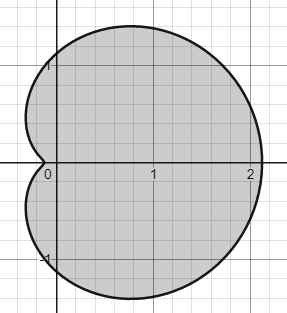
\includegraphics[scale=0.5]{cardioid}
        \end{figure}

        Clearly, there are points of $S$ in the second quadrant which are not connected by a line segment to some points of $S$ in the third quadrant, meaning that $S$ is not convex. But by construction (the polar inequality), every point in this set is connected by a line segment to the origin, so that $S$ is star convex.

        Then the product $S\times \mathbb{R}^{n-2}$ (the ``cylinder'' of $S$) is the desired subset of $\mathbb{R}^n$ which is also star convex but not convex. The origin is connected to any point $\vec{x} = (x,y,x_1,\dots,x_{n-2})$ by the line segment given by the parameterization $t\vec{x}$ for $t\in I$, but the points $(-1/4,1/2, x_1,\dots,x_{n-2})$ and $(-1/4,-1/2, x_1,\dots,x_{n-2})$ cannot be connected by a line segment.

        \item Show that if $A$ is star convex, $A$ is simply connected. 
        \begin{proof}
            Since $A$ is star convex, there exists a point $a_0$ which is connected by line segments to every point in $A$. It follows that $A$ is path connected because for any two points $a,b$ in $A$, a line segment path from $a$ to $a_0$ can be adjoined to a line segment path from $a_0$ to $b$ by the path product $\ast$ to form a path from $a$ to $b$.

            Then take any loop $P$ starting at $a_0$, and observe that for any point $a$ on the loop $P(I)$, the straight line path $ta_0 + (1-t)a$ connects $a$ with $a_0$. Hence the straight line homotopy $H\colon A\times I\to A$ given by $H(x,t) = te_{a_0}(x) + (1-t)P(x)$, where $e_{a_0}$ is the constant map into $a_0$, is the homotopy required to show that all loops in $A$ starting from $a_0$ are homotopic to a constant map into $a_0$, so that $\pi_1(A,a_0)$ is the trivial group.
        \end{proof}
    \end{enumerate}
    \item (52.2) Let $\alpha$ be a path in $X$ from $x_0$ to $x_1$; let $\beta$ be a path in $X$ from $x_1$ to $x_2$. Show that if $\gamma = \alpha \ast \beta$, then $\hat{\gamma} = \hat{\beta}\circ \hat{\alpha}$.
    \begin{proof}
        We first prove a small lemma. Socks and shoes: With $\alpha,\beta,\gamma$ as given above, we have $\overline{\gamma} = \overline{\beta}\ast \overline{\alpha}$. This is clear since \[\overline{\gamma}(t) = \gamma(1-t) = \begin{cases}
            \alpha(1-t) = \overline{\alpha}(t) & 0\leq t \leq 1/2\\
            \beta(1-t) = \overline{\beta}(t) & 1/2\leq t \leq 1
        \end{cases} = (\overline{\beta}\ast \overline{\alpha})(t)\] for all $t\in I$.

        Then for any $[f]\in \pi_1(X,x_0)$, we have $\hat{\gamma}([f]) = [\overline{\gamma}]\ast[f]\ast[\gamma] = [\overline{\beta}\ast \overline{\alpha}]\ast[f]\ast[\alpha\ast\beta]$ $= [\overline{\beta}]\ast([\overline{\alpha}]\ast[f]\ast[\alpha])\ast[\beta] = (\hat{\beta}\circ\hat{\alpha})([f])$ so that $\hat{\gamma} = \hat{\beta}\circ\hat{\alpha}$.
    \end{proof}
    \item (52.3) Let $x_0$ and $x_1$ be points of the path-connected space $X$. Show that $\pi_1(X,x_0)$ is abelian if and only if for every pair $\alpha$ and $\beta$ of paths from $x_0$ to $x_1$, we have $\hat{\alpha} = \hat{\beta}$.
    \begin{proof}
        Suppose that every pair $\alpha$ and $\beta$ of paths from $x_0$ to $x_1$ satisfies $\hat{\alpha} = \hat{\beta}$. We show that for any loops $f,g$ starting at $x_0$, that $[f]\ast [g] = [g]\ast [f]$.

        Let $\alpha$ be any path from $x_0$ to $x_1$, and choose $\beta = \overline{f}\ast \alpha$ so that \begin{align*}
            \hat{\alpha}([g]) &= [\overline{\alpha}]\ast [g]\ast [\alpha]\\
            \hat{\beta}([g]) = (\widehat{\overline{f}\ast \alpha})([g]) &= [\overline{\overline{f}\ast \alpha}]\ast [g]\ast [\overline{f}\ast \alpha] = [\overline{\alpha}]\ast[f]\ast[g]\ast[\overline{f}]\ast[\alpha]
        \end{align*}
        so that by cancellation of $[\overline{\alpha}]$ and $[\alpha]$ followed by right multiplication by $[f]$, we have that $[f]\ast [g] = [g]\ast [f]$.

        Conversely, suppose that $\pi_1(X,x_0)$ is abelian so that for any paths $f,g$ starting at $x_0$, we have $[f]\ast [g] = [g]\ast [f]$. Because $X$ is path connected, $\pi_1(X,x_0)$ is isomorphic to $\pi_1(X,x_1)$, meaning $\pi_1(X,x_1)$ is also abelian (conjugation is the trivial action).
        
        Let $\alpha,\beta$ be any two paths from $x_0$ to $x_1$. For elements $[\overline{\alpha}\ast \beta],[\overline{\alpha}\ast f\ast \alpha]\in \pi_1(X,x_1)$, we have \begin{align*}
            \hat{\alpha}([f]) = [\overline{\alpha}]\ast[f]\ast[\alpha] = [\overline{\alpha}\ast f\ast \alpha] &= [\overline{\alpha}\ast \beta]^{-1}\ast [\overline{\alpha}\ast f\ast \alpha]\ast [\overline{\alpha}\ast \beta]\\
            &=[\overline{\beta}]\ast[\alpha]\ast[\overline{\alpha}]\ast [f]\ast[\alpha]\ast[\overline{\alpha}]\ast [\beta]\\
            &= [\overline{\beta}]\ast [f]\ast [\beta] = \hat{\beta}([f]),
        \end{align*} as desired.
    \end{proof}
    \item (52.4) Let $A\subset X$; suppose $r\colon X\to A$ is a continuous map such that $r(a) = a$ for each $a\in A$. (The map $r$ is called a \textbf{\textit{retraction}} of $X$ onto $A$.) If $a_0\in A$, show that \[r_\ast \colon \pi_1(X,a_0)\to \pi_1(A,a_0)\] is surjective.
    \begin{proof} Note that the formulation of $r_\ast$ is correct because $r$ sends $a_0\in X$ to $a_0\in A$.

        For some element $[g]\in \pi_1(A,a_0)$ we seek to find a preimage of $[g]$ under $r_\ast$; that is, to find an element $[f]\in \pi_1(X,a_0)$ such that $[r\circ f] = [g]$. A choice of $f$ which works is the path given by $i_{A\xhookrightarrow{} X}\circ g$, where $i_{A\xhookrightarrow{} X}$ is the canonical inclusion map from $A$ into $X$.

        We have $r_\ast([i_{A\xhookrightarrow{} X}\circ g]) = [r\circ i_{A\xhookrightarrow{} X}\circ g] = [\id_A\circ g] = [g]$. It follows that $r_\ast$ is surjective. 

        Alternatively, we use the functorial properties of the induced homomorphism to see that since $r\circ i_{A\xhookrightarrow{} X} = \id_A$, we have that $\id_{\pi_1(A,a_0)} = (\id_A)_\ast = (r\circ i_{A\xhookrightarrow{} X})_\ast = r_\ast \circ (i_{A\xhookrightarrow{} X})_\ast$. Thus $r_\ast$ has a right inverse and so must be surjective.
    \end{proof}
    \item (52.6) Show that if $X$ is path connected, the homomorphism induced by a continuous map is independent of base point, up to isomorphisms of the groups involved. More precisely, let $h\colon X\to Y$ be continuous, with $h(x_0) = y_0$ and $h(x_1) = y_1$. Let $\alpha$ be a path in $X$ from $x_0$ to $x_1$, and let $\beta = h\circ \alpha$. Show that \[\hat{\beta}\circ (h_{x_0})_\ast = (h_{x_1})_\ast\circ\hat{\alpha}.\] This equation expresses the fact that the following diagram of maps ``commutes.''\[\begin{tikzcd}
        {\pi_1(X,x_0)} && {\pi_1(Y,y_0)} \\
        \\
        {\pi_1(X,x_1)} && {\pi_1(Y,y_1)}
        \arrow["{(h_{x_0})_\ast}", from=1-1, to=1-3]
        \arrow["{(h_{x_1})_\ast}", from=3-1, to=3-3]
        \arrow["{\hat{\alpha}}", from=1-1, to=3-1]
        \arrow["{\hat{\beta}}", from=1-3, to=3-3]
    \end{tikzcd}\]
    \begin{proof}
        Let $[f]$ be any element of $\pi_1(X,x_0)$. We apply the maps $\hat{\beta}\circ (h_{x_0})_\ast , (h_{x_1})_\ast\circ\hat{\alpha}$ to $[f]$:
        \begin{align*}
            (\hat{\beta}\circ (h_{x_0})_\ast)([f]) &= \hat{\beta}([h\circ f]) = [\overline{h\circ \alpha}]\ast [h\circ f]\ast [h\circ \alpha] = [h\circ \overline{\alpha}]\ast [h\circ f]\ast [h\circ \alpha]\\
            ((h_{x_1})_\ast\circ\hat{\alpha})([f]) &= (h_{x_1})_\ast([\overline{\alpha}]\ast[f]\ast[\alpha]) = [h\circ \overline{\alpha}]\ast [h\circ f]\ast [h\circ \alpha],
        \end{align*} where the last equalities follow from $(\overline{h\circ \alpha})(t) = (h\circ \alpha)(1-t) = h(\alpha(1-t)) = h(\overline{\alpha}(t)) = (h\circ \overline{\alpha})(t)$ and the fact that $(h_{x_1})_\ast$ is a homomorphism.
    \end{proof}
    \item (53.3) For a connected space $B$, let $p\colon E\to B$ be a covering map. Show that if $p^{-1}(b_0)$ has $k$ elements for some $b_0\in B$, then $p^{-1}(b)$ has $k$ elements for every $b\in B$. In such a case, $E$ is called a \textbf{\textit{k-fold covering}} of $B$.
    \begin{proof}Let $p\colon E\to B$ be a covering map, and let $B$ be connected.

        We prove a curious lemma first: For any positive integer $j$, the disjoint sets $S_j = \cbr{b\in B\mid \abs{p^{-1}(b)} = j}$ and $S_{\omega} = \cbr{b\in B\mid \abs{p^{-1}(b)} \text{ is infinite}}$ are open. 
        
        If $S_j$ is empty, we are done. Otherwise, for any element $x\in S_j$, there exists an evenly covered neighborhood $U_x$ of $x$ whose preimage under $p$ is the disjoint union of open sets of $E$ given by $\coprod_{\alpha} V_\alpha$. But because the preimage of $x$ under $p$ contains only $j$ elements, there are exactly $j$ open sets $V_\alpha$ which form the preimage of $U_x$. (if there are fewer, then $p$ must not be continuous). By relabeling, write $p^{-1}(U_x) = \coprod_{i=1}^j V_i$, and observe that because each $V_i$ is mapped homeomorphically into $U_x$ by $p$, it follows that $\abs{p^{-1}(y)} = j$ for every $y\in U_x$. It follows that $U_x\subseteq S_j$, so that $S_j$ is open. 
        
        The set $S_\omega$ is open due to a similar argument: Suppose $S_\omega$ is not empty, and consider $x\in S_\omega$. The preimage of an evenly covered neighborhood $U_x$ of $x$ is an infinite cardinality disjoint union of open sets $V_\alpha$ of $E$. Each $V_\alpha$ is mapped homeomorphically into $U_x$ so that the preimage of any element $y\in U_x$ is also of infinite cardinality, and thus $U_x\subseteq S_\omega$. It follows that $S_\omega$ is open, and we have proved the lemma.

        Suppose by way of contradiction that there exists (at least one) $b_1\in B$ satisfying $\abs{p^{-1}(b)} \neq k$. Observe that $b_0\in S_k$ and $b_1\in S^{\prime}= S_\omega \cup (\bigcup_{i\neq k}S_i)$, and that every element of $B$ lies in one of these two sets. Using the lemma, it follows that $S_k$ and $S^{\prime}$ are nonempty disjoint open subsets of $B$ whose union is $B$. This is impossible since $B$ is a connected space, so there are no elements in $B$ whose preimage under $p$ has cardinality not equal to $k$, as desired.
    \end{proof}
    \item (53.6b) Let $p\colon E\to B$ be a covering map. If $B$ is compact and $p^{-1}(b)$ is finite for each $b\in B$, then $E$ is compact.
    \begin{proof}
        Let $S$ be an open cover of $E$.

        Since each $b\in B$ is contained in an evenly covered open set $U_b$, the preimage of $U_b$ under $p$ is a collection $\cbr{V_{b,\alpha}}$ of disjoint open subsets of $E$ which map homeomorphically to $U_b$ by $p$. But because $p^{-1}(b)$ is finite, it follows that $\cbr{V_{b,\alpha}}$ is finite (that is, $\alpha$ takes on finitely many values). Relabeling, write the collection as $\cbr{V_{b,1}, \dots, V_{b,\abs{p^{-1}(b)}}}$.

        Since $E$ is covered by $S$, we can find open sets $S_{b,1}, \dots, S_{b,\abs{p^{-1}(b)}}$ from $S$ such that $S_{b,\alpha}$ contains the point $p^{-1}(b)\cap V_{b,\alpha}$ (the single element of the preimage of $b$ under $p$ lying in the $\alpha$-th slice $V_{b,\alpha}$). We apply $p$ to each of the intersections $S_{b,1}\cap V_{b,1}, \dots, S_{b,\abs{p^{-1}(b)}}\cap V_{b,\abs{p^{-1}(b)}}$ to produce a family of neighborhoods of $b$ which lie in $U_b$ given by $\cbr{p(S_{b,\alpha}\cap V_{b,\alpha})}_{\alpha = 1}^{\abs{p^{-1}(b)}}$, and so we take the (finite) intersection over this family to produce a small neighborhood $W_b$ of $b$ contained in $U_b$: \[W_b = \bigcap_{\alpha = 1}^{\abs{p^{-1}(b)}}p(S_{b,\alpha}\cap V_{b,\alpha}).\]

        Since $b$ was arbitrary, the collection $W = \cbr{W_b}$ for all $b$ constitutes an open cover of $B$, and by compactness of $B$ we can find a finite subcover $W^{\prime} = \cbr{W_{b_n}}_{n=1}^{N}$ of $B$. Note that the preimage of each $W_b$ is contained in each $S_{b,\alpha}$ for $1\leq \alpha \leq \abs{p^{-1}(b)}$. It follows also that the preimage of each $W_b$ is contained in the union $\bigcup_{\alpha = 1}^{\abs{p^{-1}(b)}}S_{b,\alpha}$ (the union is bigger than the intersection).

        With $W^{\prime}$ being a finite subcover of $B$, we have that \begin{align*}
            E = p^{-1}(B)\subseteq p^{-1}\br{\bigcup_{n=1}^N W_{b_n}} \subseteq \bigcup_{n=1}^N \sbr{\bigcup_{\alpha = 1}^{\abs{p^{-1}(b_n)}}S_{b_n,\alpha}},
        \end{align*}
        where the last set is a finite union of open sets of $S$ so that $S$ admits a finite subcover of $E$. Since $S$ was an arbitrary open cover of $E$, it follows that $E$ is compact.
    \end{proof}
\end{enumerate}
\end{document}